\documentclass{article}
\usepackage{neurips_2026}
\usepackage[utf8]{inputenc}
\usepackage[T1]{fontenc}
\usepackage{hyperref,url,booktabs,amsfonts,microtype,xcolor,graphicx}
\title{Mechanical Validity Does Not Imply World-Model Fidelity:\\Evaluating LLM-Generated Executable POSGs}
\author{PRISM Fellowship Team}

\begin{document}
\maketitle

\begin{abstract}
World models used for planning must capture action-conditioned dynamics, not
merely satisfy an executable interface. We study whether large language models
can translate natural-language situations into executable partially observable
stochastic games (POSGs). Our repository contains 44 scenarios spanning toy,
situational, game, and cultural settings; the controlled experiment reported
here evaluates five model families on nine finite games with three independent
runs per model--game pair (135 final artifacts). First-pass mechanical validity
is 124/135 (91.85\%) and varies from 81.48\% to 100\% by model; recorded repair
rounds produce valid artifacts for all 135 trials. Yet the 134 artifacts that
pass a subsequent Lane-1 audit obtain mean structural F1 0.7178, and only 32
are exact matches under the implemented feature-multiset comparison. Because
the optimal graph-matching dependency was unavailable, we report this score as
a representation-sensitive fallback rather than semantic equivalence. The
results empirically support a three-level distinction: executable models can be
mechanically valid without reproducing reference transition structure, while
semantic faithfulness requires separate evidence.
\end{abstract}

\section{Introduction}
World models mediate what a planning agent believes is reachable, reversible,
or risky. A generated simulator may parse and execute while omitting an action,
inventing stochasticity, terminating prematurely, or assigning the wrong
successor. Such errors alter the induced transition system and therefore any
downstream quantity computed from it.

We evaluate LLMs as translators from natural-language situations to formal
POSGs. Our central message is \emph{executable $\neq$ structurally faithful
$\neq$ semantically faithful}. We ask: (RQ1) how reliably do models produce
mechanically valid POSGs; (RQ2) how closely do valid outputs reproduce
reference-backed state/action/transition features; and (RQ3) how stable is
generation across three repeated runs?

Our contributions are: (1) a 44-scenario benchmark and JSON/Python generation
pipelines; (2) a three-lane evaluation separating mechanical validity,
structural comparison, and semantic diagnostics; (3) a five-model, nine-game,
three-run empirical comparison with complete prompts, replies, repairs, probes,
and serialized graphs; and (4) a reproducible conditional analysis showing
that mechanical success alone does not establish structural fidelity.

\section{Related Work}
Our work connects formal stochastic-game modeling, program synthesis by LLMs,
and evaluation of learned world models. Unlike pixel-prediction benchmarks, we
study symbolic action-conditioned dynamics whose reachable transition graph can
be enumerated. This controlled setting complements embodied world-model work:
it exposes formal errors precisely, but does not establish physical realism or
control performance.

\section{Benchmark and World-Model Generation}
The benchmark contains 10 toy, 11 situational, nine game, and 14 cultural
scenarios. The main controlled study uses G1--G9: Rock--Paper--Scissors, dice
and coin games, penalty kick, matching pennies, auction, Prisoner's Dilemma,
Stag Hunt, and a small Colonel Blotto game. These are symbolic controls rather
than a Physical-AI benchmark.

Each model receives the same Python POSG contract. It must define players,
initial state, legal actions, transition distributions, observations, rewards,
and terminal detection. The harness executes the code, exhaustively enumerates
reachable states within configured bounds, and exports canonical JSON and a
graph. Failed mechanical attempts may receive explicitly logged repair rounds;
first-pass and repair-assisted rates are reported separately.

\section{Evaluation Framework}
\paragraph{Lane 1: mechanical validity.}
Checks cover execution, hashable states, the interface contract, probability
distributions, references, joint-action completeness, reachability, and paths
to termination.

\paragraph{Lane 2: structural fidelity.}
Candidates are compared with reference POSGs using feature coverage, precision,
and their harmonic mean. The external optimal \texttt{game\_matching} package
was unavailable during evaluation, so all 135 rows use the documented
feature-multiset fallback. This comparison is sensitive to modeling granularity:
a richer outcome expansion can reduce precision without being semantically
wrong. We therefore call the result \emph{fallback structural F1}, not a
semantic score.

\paragraph{Lane 3: semantic diagnostics.}
Automated checklists inspect actor/action coverage and flag text for review.
They are not human ground truth; a checklist pass or bias flag is not evidence
of semantic correctness or bias. Lane 3 is not used as the main outcome here.

\section{Experimental Setup}
We evaluate GPT-5.6 Sol, Claude Opus 5, Llama 3.3 70B Instruct, Qwen 3.8 27B,
and DeepSeek V4 Flash through OpenRouter. Each model is run once on each of nine
games in each of three preserved runs, yielding 27 trials per model and 135
final artifacts. The run directories retain configuration, exact prompts, raw
responses, generated Python, probe reports, canonical JSON, and graph objects.
The study is zero-shot at first pass; repair attempts are part of the harness
and separately counted. We do not pool the earlier local-Qwen, prompt-variant,
or robustness experiments because their conditions differ.

\section{Results}
\subsection{RQ1: Mechanical validity}
Across all trials, 124/135 (91.85\%) succeed on the first attempt. All 135
eventually produce contract-valid artifacts after recorded repair rounds. A
post-hoc Lane-1 evaluation passes 134/135; the sole failure is DeepSeek G9 in
run 1. This distinction matters: final generation validity is the harness's
repair outcome, whereas Lane 1 is a later, stricter audit.

\begin{table}[t]
\centering
\caption{Mechanical reliability and fallback structural comparison across 27
trials per model. Structural values are means; $\pm$ is sample SD over the 27
model--game--run rows.}
\label{tab:main}
\small
\begin{tabular}{lrrrrr}
\toprule
Model & First pass & L1 & Coverage & Precision & Structural F1 \\
\midrule
Claude Opus 5 & 27/27 & 27/27 & .9083 & .4112 & $.5175\pm.3101$ \\
DeepSeek V4 Flash & 23/27 & 26/27 & .7788 & .7334 & $.7071\pm.2868$ \\
GPT-5.6 Sol & 26/27 & 27/27 & .9440 & .7625 & $.7854\pm.3043$ \\
Llama 3.3 70B & 22/27 & 27/27 & .8891 & .7018 & $.7487\pm.2338$ \\
Qwen 3.8 27B & 26/27 & 27/27 & .8577 & .8762 & $.8221\pm.2507$ \\
\bottomrule
\end{tabular}
\end{table}

\begin{figure}[t]
\centering
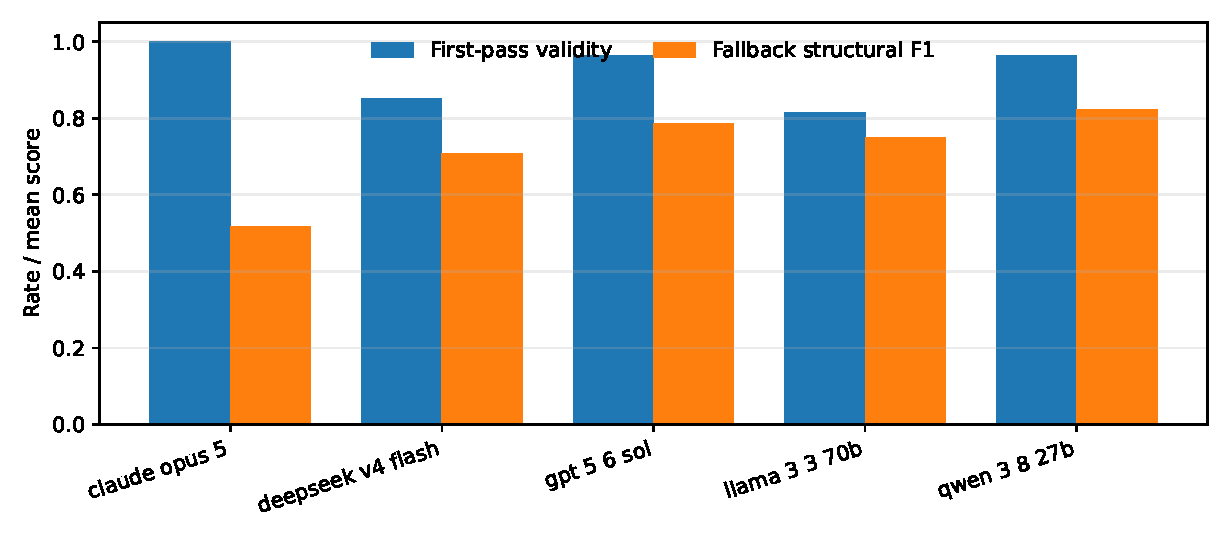
\includegraphics[width=\linewidth]{figures/main_empirical_results.pdf}
\caption{First-pass mechanical validity and mean fallback structural F1 by
model (27 trials each). The two quantities are not interchangeable: validity
is a pass rate, whereas structural F1 compares reference/candidate feature
multisets and is sensitive to representation granularity.}
\label{fig:main-results}
\end{figure}

\subsection{RQ2: Structural fidelity conditional on validity}
The mean fallback structural F1 over all 135 evaluated artifacts is 0.7162.
Among the 134 Lane-1-passing artifacts it is 0.7178; only 32/134 attain F1=1
under the fallback. Thus, the mechanical gate removes almost none of the broad
structural variation. Table~\ref{tab:main} also shows why coverage alone is
insufficient: Claude has high mean coverage but low precision, consistent with
extra represented features or finer granularity. We do not label every feature
difference an error without case-level semantic inspection.

\subsection{RQ3: Observed run-to-run reliability}
First-pass validity falls from 43/45 (95.56\%) in run 1 to 41/45 (91.11\%) in
run 2 and 40/45 (88.89\%) in run 3. By model it ranges from 22/27 (81.48\%) for
Llama to 27/27 (100\%) for Claude, with DeepSeek at 23/27 and GPT/Qwen at
26/27. Three repetitions reveal generation variability but are too few for
claims of statistical significance or stable population rankings. The large
per-model structural SDs in Table~\ref{tab:main} mix case difficulty and run
variation and should not be read as a pure stability estimator.

\subsection{Separate cultural diagnostic}
A separate dataset contains 84 JSON candidates: three models, 14 cultural
cases, and anonymized versus country-named prompts, one sample per cell. Strict
parsing succeeds for 26/28 GPT outputs and 26/28 Claude outputs but 0/28 Llama
outputs; lenient recovery obtains 26/28 and 28/28 Llama candidates in the two
conditions. Mean automated semantic scores change by only $-0.006$, $-0.007$,
and $-0.001$ when location is revealed for GPT, Llama, and Claude respectively.
These are descriptive diagnostics: providers differ for Llama across
conditions, there is one sample per cell, and no human annotation validates the
automated semantic or bias checks.

\section{Discussion and Failure Analysis}
Mechanical correctness is necessary but insufficient for a trustworthy
executable world model. The conditional analysis demonstrates the logical gap:
nearly every artifact passes Lane 1, while fallback structural scores span a
wide range. Observed differences can reflect under-modeling (missing features
or shortened trajectories), over-modeling (extra states or finer outcome
expansion), transition/terminal differences, or merely alternative but valid
granularity. Only reference mechanics and targeted semantic checks can
distinguish those explanations.

For safety-relevant use, an omitted successor can make a harmful state appear
unreachable; an invented reverse edge can make an irreversible action appear
recoverable; and incorrect stochasticity changes risk estimates. Our experiments
show that such formal evaluation is needed, not that these symbolic models are
safe for deployment. No downstream planner or controller is evaluated.

\section{Limitations}
The main benchmark has nine small symbolic games, not continuous or perceptual
physical dynamics. There are only three repetitions per model--game pair, and
provider/model versions may change. Exhaustive rollout is bounded. Lane 2 uses
a representation-sensitive feature fallback because optimal graph matching was
unavailable; topology alone does not establish semantic correctness. Human
Lane-3 annotation is incomplete, so automated semantic scores and flags remain
diagnostic. The situational Python artifacts lack a compatible completed
aggregate evaluation, and the v3 JSON track was authored offline by hand, so
neither is reported as LLM performance. Finally, we do not measure downstream
planning, control, empowerment, or real-world safety.

\section{Conclusion}
We evaluated five LLMs across nine formal games and three runs, preserving 135
auditable executable POSGs. First-pass validity is high but imperfect and
varies across models and runs; repair makes all artifacts executable, while a
later mechanical audit passes 134. Structural comparison remains substantially
below exact agreement for most mechanically valid models. The empirical lesson
is narrow but important: executability is a gate, not evidence of world-model
fidelity. Future work should add embodied dynamics, validated human semantic
annotation, representation-invariant matching, and downstream policy tests.

\end{document}
